\chapter{Testovanie a vyhodnocovanie}
\label{chap:testovanie-vyhodnocovanie}
Po naimplementovaní navrhnutého riešenia, ktoré bolo popísané v kapitole \ref{chap:implementacia}, nasledovalo testovanie a vyhodnocovanie, ktorému sa venuje práve táto kapitola.  Kapitola začína popisom testovania serverového aplikačného riešenia pomocou testovacieho rámca Tavern, pokračuje testovaním užívateľského rozhrania aplikácie a vyhodnocovaním naimplementovanej detekcie chronických rán. Na záver kapitoly sú zhrnuté ďalšie možné vylepšenia práce a je načrtnuté budúce smerovanie projektu. 

%%%%%%%%%%%%%%%%%%%%%%%%%%%%%%%%%%%%%%%%%%%%%%%%%%%%%%%%%%%%%%
\section{Testovanie serverového aplikačného rozhrania}
Testovanie aplikačného rozhrania prebiehalo už počas samotnej implementácie, kedy vždy po naprogramovaní nejakej sady koncových adries, boli napísané aj testy na overenie funkcionality týchto adries. Testovanie prebiehalo pomocou Python testovacieho rámca Tavern, ktorý je voľne dostupný pod licenciou MIT. Tavern je plugin pre Pytest, nástroj príkazovej riadky a aj Pythonova knižnica v jednom určená pre testovanie aplikačných rozhraní založených nielen na RESTe. Používa syntax založenú na YAML, ktorá je veľmi flexibilná a jednoduchá. Okrem RESTful aplikačných rozhraní dokáže testovať aj rozhrania založené na MQTT. Veľká výhoda Tavern je, že môže byť veľmi jednoducho použitý v hocijakom continous integration procese. \cite{AXUaooptJGOSpUrX} 

Testy vytvorené pre Tavern sú teda definované v YAML súboroch, ktoré predstavujú danú testovaciu sadu. Táto sada je vždy definovaná svojím menom (\textit{test\_name}) a jednotlivými krokmi samotného testu (\textit{stages}).  Každý jeden krok predstavuje samostatné dotazovanie sa na server a volanie serverovej funkcie. Kroky sa skladajú z mena kroku (\textit{name}), z požiadavky (\textit{request}), ktorá sa vykonáva a z odpovede (\textit{response}), ktorá sa kontroluje. V požiadavke je možné definovať všetky nastavenia, ako url adresy serveru (\textit{url}), na ktorý sa bude posielať požiadavka, metódu, ktorá sa bude vykonávať (\textit{method}), dáta vo formáte json, ktoré sa na server budú odosielať (\textit{json}) a prípadne ďalšie hlavičky (\textit{headers}), ktoré sú v požiadavke prítomné (v tomto prípade je prítomná iba hlavička \textit{Authorization}). Správnosť odpovede, ktorá sa potom vyhodnocuje je overovaná podľa vráteného stavového kódu (\textit{status\_code}) a dát obsiahnutých v tele (\textit{body}), poprípade iných položiek, ktoré ale v prípade tejto práce nie sú potrebné. Štruktúru takéhoto kroku testu je možné vidieť pre predstavu v kóde. 
\begin{lstlisting}[caption={Ukážka testovacieho kroku.},captionpos=b]
...
- name: Get scale list after update
    request:
      url: "{env_host:s}/scale"
      method: GET
      headers:
        Authorization: "{firebase_token:s}"
    response:
      status_code: 200
      body:
        - name: Scale
          unit: px
          value: 10
          user: "{firebase_user:s}"
          _id:
            \$oid: "{scale_id:s}"
...
\end{lstlisting}
Testy sú spúšťané pomocou nástroju príkazového riadku Tavern-CI. Testy tejto práce boli rozdelené do 2 súborov, a to na prípady, ktoré môžu nastať pri každodennom používaní aplikácie (\textit{valid.tavern.yaml}) a na prípady, ktoré by mohli nastať iba v prípade nejakej neočakávanej chyby, alebo pri pokuse o hackovanie aplikácie (\textit{invalid.tavern.yaml}). Súbor \textit{enviroment.yaml} slúži na uchovávanie premenných, ktoré sa používajú a sú vkladané do obidvoch testov. Ide o premennú kľúča k Firebase Authentification, e-mailu a hesla k účtu testovacieho užívateľa a koreňovú adresu serveru aplikačného rozhrania. Kroky testu sa vyhodnocujú postupne a v prípade, že sa nevyhodnotí správne jeden krok, tak vyhodnocovanie ďalších krokov je zrušené a užívateľ je o tejto skutočnosti informovaný. Po otestovaní finálnej podoby aplikačného serverového rozhrania, kedy všetky testy dopadli úspešne, bolo toto rozhranie považované za stabilné a fungujúce správne. 

%%%%%%%%%%%%%%%%%%%%%%%%%%%%%%%%%%%%%%%%%%%%%%%%%%%%%%%%%%%%%%
\section{Vyhodnocovanie detekcie chronickej rany}
Vyhodnocovanie a testovanie poloautomatickej detekcie bolo vykonávané na snímkoch chronických rán, ktoré poskytla Fakultná nemocnica Brno. Ide o snímky vytvorené pomocou bežného mobilného fotoaparátu, ktorý nebol ničím špeciálny a nachádza sa takmer v každom modernom mobilnom zariadení. Získavanie snímok neprebiehalo za prítomnosti žiadnych špeciálnych predpripravených podmienok. Snímky sú rôznej kvality a zachycujú rôzne chronické rany v rôznych štádiách, od rán, ktoré sa skoro neprejavili, až po rany, ktoré už boli v pokročilom štádií a značne komplikované ako na liečbu, tak aj na samotnú detekciu. Snímky boli získavané nemocnicou približne od polovice januára 2018 do polovice mája 2018 a takto bolo získaných 40 snímok zo 14 unikátnych defektov (v rovnakom čase bol ten istý defekt zachytený niekoľkokrát). Z týchto 14 defektov sa avšak nejednalo vždy o chronické rany, ale objavila sa aj snímka stareckých škvŕn, alebo jedno približne 60 ročné materské znamienko. Unikátnych chronických rán bolo teda dokopy 12 a z toho 10 bolo použitých pre vyhodnocovanie. Všetky unikátne rany boli autorom práce anotované za pomoci externého konzultanta tejto práce.

Výskumy, ktoré sa zaoberali detekciou chronických rán, alebo príbuzných defektov a boli behom práce na tomto projekte preštudované, boli vykonávané pod určitými kontrolovanými podmienkami, ako napríklad špeciálne nasvietenie rany a podobne (štúdie \cite{4353723}, \cite{6461344} a \cite{6399754}). Detekcia a analýza iných rán zase prebiehala iba na ručne predspracovaných snímkach, napríklad bez pozadia, alebo snímkach, ktoré obsahovali iba samotnú ranu (štúdie \cite{5286322} a \cite{6306219}). Iné štúdie ako \cite{6172044} alebo \cite{6392633} sa zase zamerali iba na určitý špecifický typ chronickej rany. Všetky tieto štúdie boli overované na dátovej sade obsahujúcej od 5 v \cite{6172044} do 113 snímkov v \cite{5286322}. Ich presnosť detekcie za týchto, dá sa povedať zjednodušených podmienok, dosahovala presnosť od 56,4\% v \cite{4353723} do 98\% v \cite{6306219}. Dá sa ale predpokladať, že takéto podmienky pri získavaní snímok pomocou mobilného zariadenia v bežnej lekárskej praxi nastať nemôžu, alebo iba veľmi ťažko. Sťažením tohoto projektu oproti spomenutým štúdiám bolo avšak to, že snímky neboli získavané behom žiadnych kontrolovaných podmienok, neboli ručne predspracované a taktiež kvôli nedostatku testovacieho materiálu bola práca zameraná na všetky typy chronických rán, nie iba na niektorých špecifických. 

Samotné vyhodnocovanie a testovanie bolo vykonávané tak, že testovacie snímky boli manuálne ohraničené externým konzultantom z nemocnice pomocou špeciálne vytvorenej webovej aplikácie pre tieto účely, ktorú je možné vidieť na obrázku \ref{fig:anotator} a tak vznikli akési predlohy na porovnávanie a vyhodnotenie poloautomatickej detekcie. 
\begin{figure}[h]
  \centering
  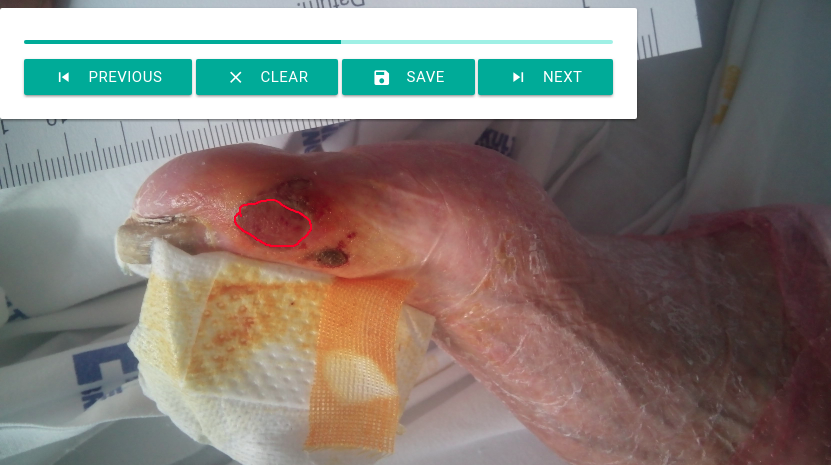
\includegraphics[scale=0.5]{fig/anotator.png}
  \caption{Webová aplikácia na ohraničovanie snímok konzultantom.}
  \label{fig:anotator}
\end{figure}
Je nutné podotknúť, že chronické rany sú veľmi zložité a keď sa stretne viacero špecialistov, tak môžu mať rozdielny názor na to, čo ešte patrí do priestoru rany a čo už rana nieje. Je teda nutné pri detekcií a aj tvorbe predlohy a porovnávaní s ňou vždy rátať s určitou dávkou subjektivity. Rany na snímkach boli potom detekované pomocou poloautomatickej metódy detekcie. Po detekcií boli hodnoty vypočítaného obsahu rany a očakávaného obsahu v pixeloch navzájom porovnávané. Výsledky je možné vidieť v tabuľke \ref{tab:result}, kde je vždy uvedené číslo rany, ktoré odpovedá menu súboru z priečinku \textit{shots/eval} nachádzajúceho sa na priloženom nosiči. Úspešnosť detekcie je vždy vyjadrená číselne v pixeloch a v percentách. Okrem úspešnosti detekcie je prítomný aj stĺpec, ktorý hovorí, koľko pixelov na obrázku bolo klasifikovaných nesprávne ako pixel chronickej rany. 
\begin{table}[h]
\centering
\label{tab:result}
\begin{tabular}{|l|l|l|l|l|}
\hline
Rana & Detekované & Očakávané & Správne detekované & Nesprávne detekované \\ \hline
1    & 6280px               & 13820px           & 6213px (44.96\%)    & 67px         \\ \hline
2    & 0px                  & 261px             & 0px (0.00\%)        & 0px          \\ \hline
3    & 1108px               & 10296px           & 1041px (10.11\%)    & 67px         \\ \hline
4    & 10484px              & 2244px            & 2244px (100.00\%)   & 8240px     \\ \hline
5    & 7499px               & 8285px            & 5424px (65.47\%)    & 2075px      \\ \hline
6    & 3026px               & 2495px            & 2038px (81.68\%)    & 988px       \\ \hline
7    & 46712px              & 34051px           & 34046px (99.99\%)   & 12666px     \\ \hline
8    & 6307px               & 7182px            & 6161px (85.78\%)    & 146px        \\ \hline
9    & 23917px              & 2301px            & 2301px (100.00\%)   & 21616px    \\ \hline
10   & 5509px               & 6560px            & 5022px (76.55\%)    & 487px        \\ \hline
\end{tabular}
\caption{Výsledky vyhodnocovania poloautomatickej detekcie}
\end{table}
V tabuľke výsledkov je možné si všimnúť, že výsledné hodnoty boli rôzne, tak ako jednotlivé rany. Behom práce bolo navrhnuté, aby sa projekt zameral len na určitý druh rán v určitom štádií, vzhľadom na to, aké až príliš rozdielne boli jednotlivé rany na snímkach. Bohužiaľ ale behom pol roka nebolo možné získať taký dostatočný počet snímkov, aby sa bolo možné užšie zameranie. Z obrázkov je jasné, že čo rana to v podstate iný druh v inom štádií a preto boli v rámci implementácie zvolené postupy také aké boli, teda okrem poloautomatickej detekcie algoritmom Region Growing bol pridaný aj manuálny mód ohraničenia rany. Z tabuľky je možné si všimnúť hodnoty úspešnosti detekcie, ktoré sú presne 100\%. Rany, ktoré majú takúto úspešnosť boli síce detekované celé, avšak do okolia rany bol zahrnutý aj predstupeň pred samotným defektom. Takúto ranu je možné vidieť na obrázkoch \ref{fig:w4} a \ref{fig:w4d}. Naopak veľmi dobre bola detekovaná rana, ktorá bola jasne iná ako okolitá pokožka a to tak, že aj lajk by dokázal ranu ohraničiť. Ranu je možné vidieť na obrázkoch \ref{fig:w8} a \ref{fig:w8d}.

%%%%%%%%%%%%%%%%%%%%%%%%%%%%%%%%%%%%%%%%%%%%%%%%%%%%%%%%%%%%%%
\section{Ďalšie smerovanie projektu}
Ako je možné zistiť podľa výsledkov, tak poloautomatická detekcia funguje rôzne na rôznych snímkach. Zatiaľ čo funguje na ranách, ktoré sú farebne dobre oddelené od okolitej kože, tak podstatne viac zlyháva na ranách, ktoré sú menej výrazné, alebo sú pomerne komplikované. Avšak, aby boli tieto tvrdenia potvrdené, je nutné urobiť ďalšiu a oveľa väčšiu sadu snímkov, a keďže behom 5 mesačného obdobia bolo bolo zaznamenaných 12 unikátnych defektov, typu chronická rana, tak tento proces bude nezanedbateľne časovo náročný. Z toho dôvodu nie je úplne overená funkčnosť poloautomatickej detekcie. Aplikácia však môže byť využívaná, tak, že sa bude používať poloautomatická detekcia na pomerne jednoduchších a farebne výraznejších ranách, a na zložitejších ranách bude využívaná manuálna detekcia pomocou ohraničenia rany prstom/myšou. Okrem toho, že poloautomatická detekcia bola testovaná na chronických ranách, tak bola testovaná aj na pár snímkach hematómov a jednom výraznom znamienku, ktoré nemocnica taktiež poskytla. Ako je vidieť na obrázkoch \label{fig:w2} a \label{fig:w3}, tak aplikácia môže byť použitá aj na takéto prípady. Poprípade sa môže algoritmus ľahko upraviť, aby mohli byť detekované všetky tieto prípady, keďže hematómy sú v porovnaní s chronickými ranami oveľa menej rozmanité a teda viac farebne navzájom podobné.
\begin{figure}[h]
   \begin{minipage}{0.4\textwidth}
     \centering
     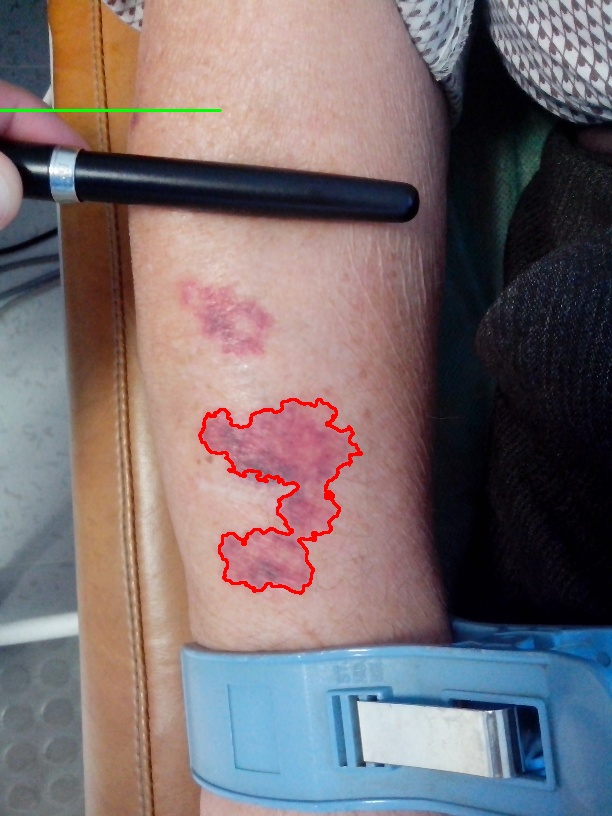
\includegraphics[scale=0.35]{fig/2o.jpeg}
      \caption{Detekcia hematómu.}
      \label{fig:w2}
   \end{minipage}\hfill
   \begin{minipage}{0.4\textwidth}
     \centering
     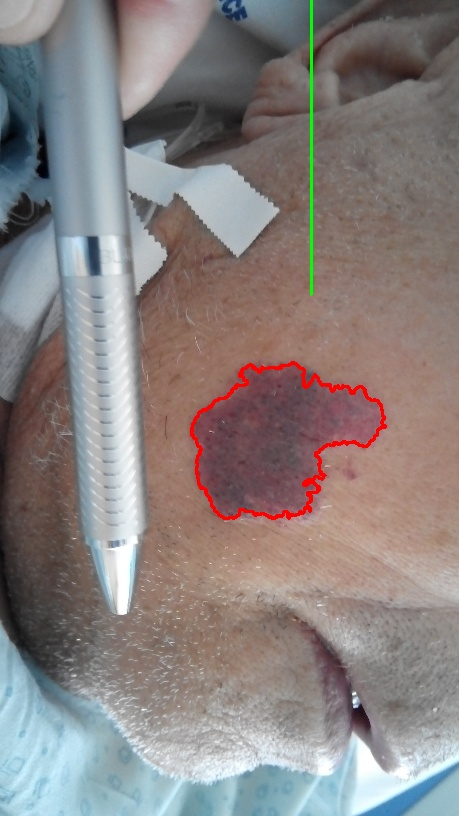
\includegraphics[scale=0.35]{fig/3o.jpeg}
      \caption{Detekcia znamienka.}
      \label{fig:w3}
   \end{minipage}
\end{figure}

\begin{figure}[h]
   \begin{minipage}{0.48\textwidth}
     \centering
     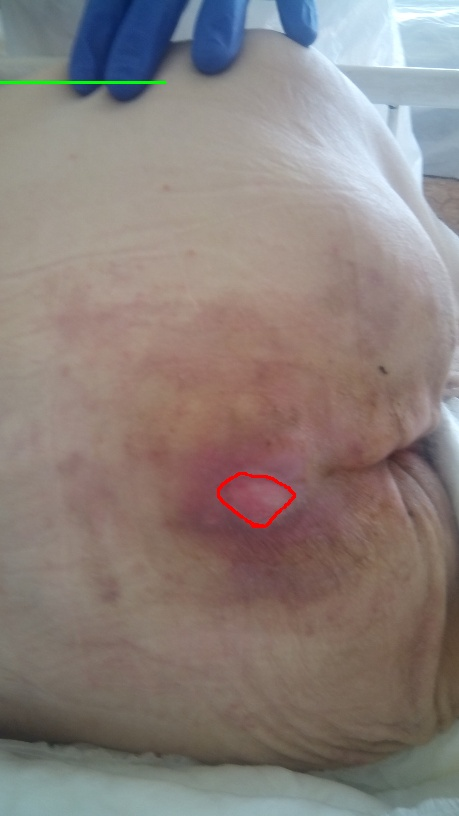
\includegraphics[scale=0.35]{fig/4m.jpeg}
      \caption{Rana 4 - manuálna detekcia, očakávaná.}
      \label{fig:w4}
   \end{minipage}\hfill
   \begin{minipage}{0.48\textwidth}
     \centering
     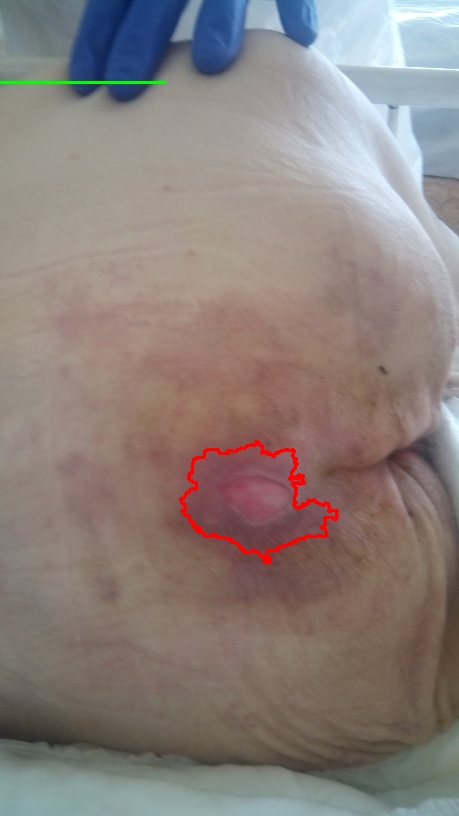
\includegraphics[scale=0.35]{fig/4a.jpeg}
      \caption{Rana 4 - automatická detekcia.}
      \label{fig:w4d}
   \end{minipage}
   \break \break \break
   \begin{minipage}{0.48\textwidth}
     \centering
     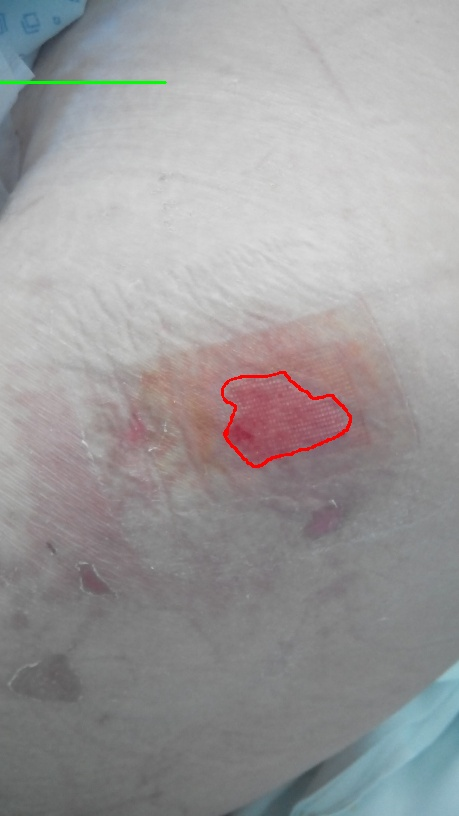
\includegraphics[scale=0.35]{fig/8m.jpeg}
      \caption{Rana 8 - manuálna detekcia, očakávaná.}
      \label{fig:w8}
   \end{minipage}\hfill
   \begin{minipage}{0.48\textwidth}
     \centering
     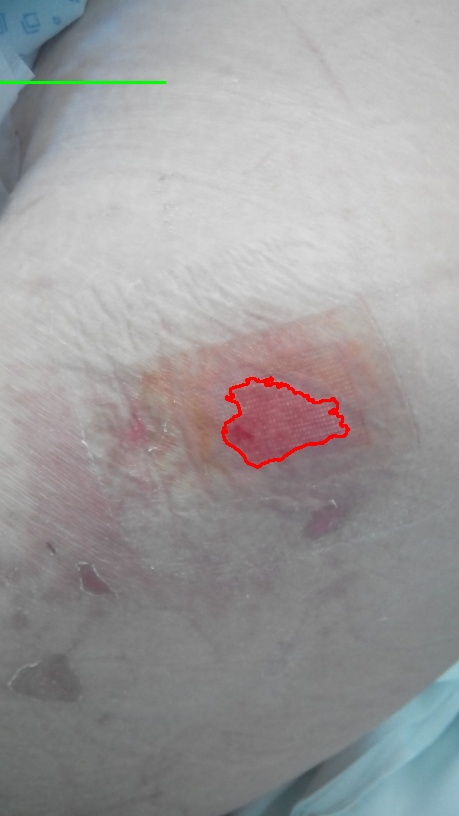
\includegraphics[scale=0.35]{fig/8a.jpeg}
      \caption{Rana 8 - automatická detekcia.}
      \label{fig:w8d}
   \end{minipage}
\end{figure}